\subsubsection{Spielgerät}

Die Spielgeräte wurden von Kevin Cornelius entworfen und von ihm und Rafael Hadamik gebaut.
Das Spielgerät, nachfolgend genannt "Tagger", ist eine Infrarot-Pistole inklusive Empfänger. Die einzelnen Spieler benötigen beim Spielen des Lasertags nur den "Tagger" und keine Weste. Deshalb bleiben sie voll beweglich und es erhöht gleichzeitig den Schwierigkeitsgrad. \\
Bei der Wahl der Materialien musste man vor allem das Budget, die Stabilität und die Handhabung berücksichtigen, damit ein vernünftiges Spiel enstehen kann. Daraus folgt der grundlegende Aufbau des "Taggers":
\begin{enumerate}
	\item Die Schaltungen wurden mit einzelnen Komponenten, Jumper-Kabeln und Lochrasterplatten gesteckt und gelötet.
	\item Die Infrarot-LED wird durch ein Aluminiumrohr gerichtet, damit ein gebündelter Infrarot-Strahl entsteht und die natürliche Streuung eines Infrarot-Signals nicht das Spielen erschwert.
	\item Als Rechensystem wurde ein Raspberry Pi Zero W benutzt, dieser  hat die oben beschriebenen Anforderungen am Besten erfüllt.
	\item Der Akkumulator konnte aufgrund des geringen Stromverbrauches mit geringer Kapazität, kleinen Abmessungen und geringem Preis gewählt werden.
	\item Das Gehäuse des "Taggers" wurde mit Acrylglas und der Benutzung geeigneter Werkzeuge hergestellt. Acrylglas ist sehr bruchsicher und leicht, was beides sehr geeignete Eigenschaften für dieses Gehäuse sind.
\end{enumerate}
\begin{figure}[ht]
	\centering
		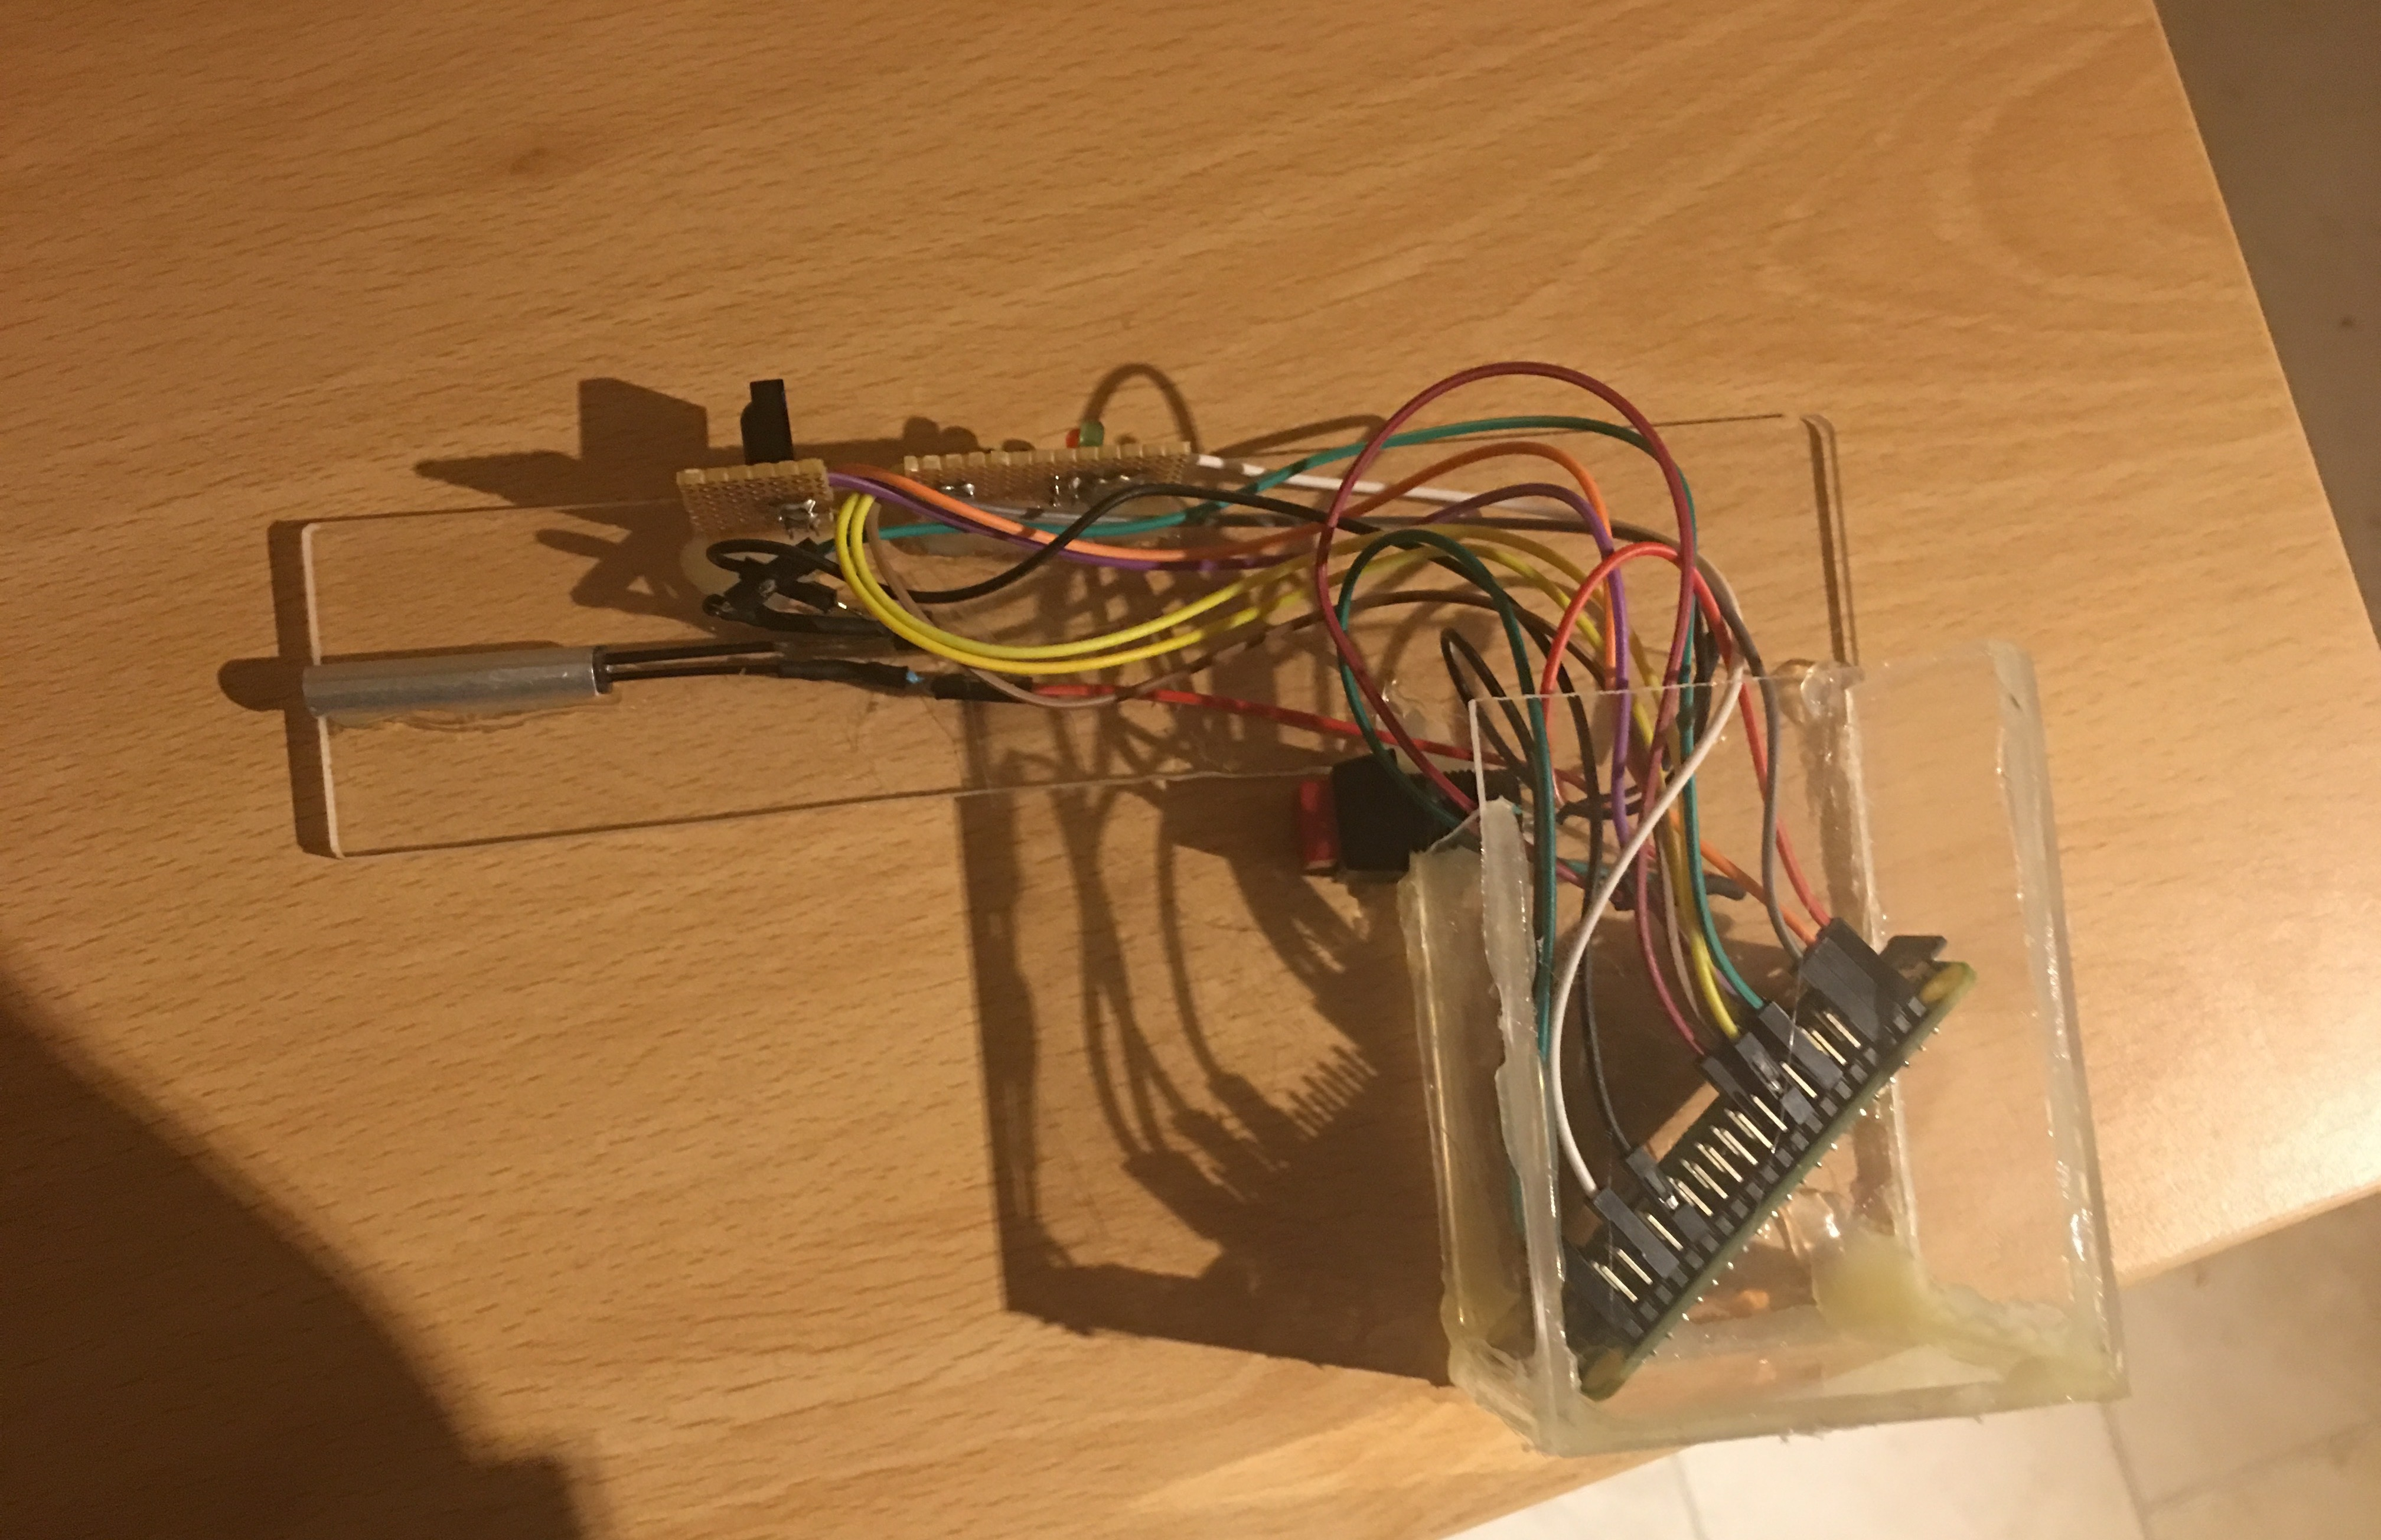
\includegraphics[width=0.7 \textwidth]{./040-komponenten/010-hardware/tagger.jpg}
	\caption{Das Spielgerät}
	\label{fig:Bild1Hardware}
\end{figure}

